% Created 2019-11-14 jue 22:00
\documentclass[letterpaper]{scrartcl}
\usepackage[utf8]{inputenc}
\usepackage[T1]{fontenc}
\usepackage{fixltx2e}
\usepackage{graphicx}
\usepackage{longtable}
\usepackage{float}
\usepackage{wrapfig}
\usepackage{rotating}
\usepackage[normalem]{ulem}
\usepackage{amsmath}
\usepackage{textcomp}
\usepackage{marvosym}
\usepackage{wasysym}
\usepackage{amssymb}
\usepackage{hyperref}
\tolerance=1000
\usepackage{khpreamble}
\usepackage{geometry}
\geometry{top=20mm, bottom=20mm, left=22mm, right=18mm}
\author{Kjartan Halvorsen}
\date{\today}
\title{State feedback with observer exercise}
\hypersetup{
  pdfkeywords={},
  pdfsubject={},
  pdfcreator={Emacs 25.3.50.2 (Org mode 8.2.10)}}
\begin{document}

\maketitle

\subsection*{Complete the block diagram}
\label{sec-0-1}
\begin{center}
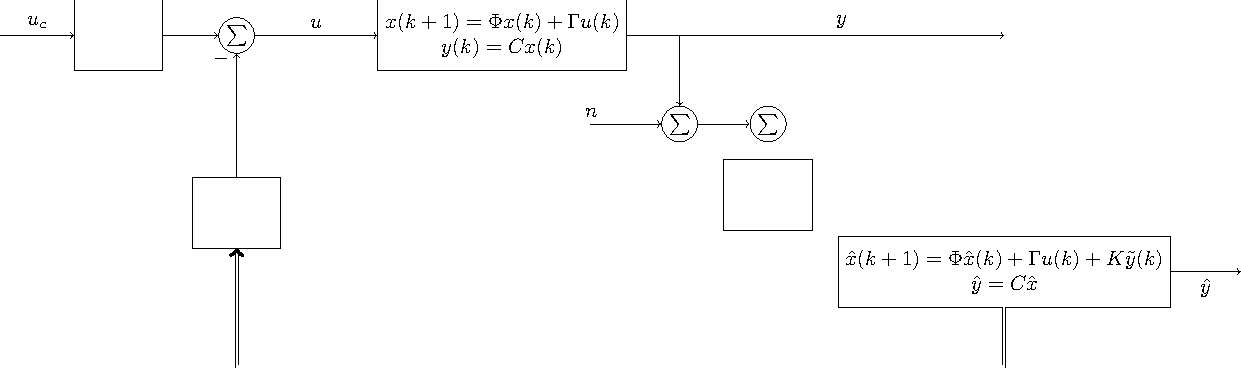
\includegraphics[width=\linewidth]{../../figures/state-feedback-with-observer-incomplete}
\end{center}

The control law is \(u(k) = l_0u_c(k) - L\hat{x}(k)\). The feedback to the observer is \(K\tilde{y}(k) = K\big(y_m(k) - \hat{y}(k)\big) = K\big(y(k) + n(k) - C\hat{x}(k)\big) \) 


\subsection*{Complete the augmented state-space model}
\label{sec-0-2}

\begin{align*}
\bbm x(k+1)\\\hat{x}(k+1) \ebm &= \bbm & & & & & & & &&& & & &\\ &&& & & & & & & & & & &\ebm \bbm x(k)\\\hat{x}(k)\ebm + \bbm &&&\\&&&\\&&&\\&&& \ebm u_c(k) + \bbm &&&\\&&&\\&&&\\&&& \ebm n(k)\\
y(k) &= \bbm &&&&&& \ebm \bbm x(k)\\\hat{x}(k)\ebm
\end{align*}

\newpage

\subsection*{Control of a tank model}
\label{sec-0-3}
Consider the system of two tanks in the figure below. The input signal is the flow of water into the upper tank, and the output signal is the level of the second tank. 

\begin{minipage}{0.6\linewidth}
In continuous-time the system is described by the state space system
\begin{align*}
\frac{dx}{dt} &= \bbm -0.0197 & 0\\0.0178 & -0.0129 \ebm x + \bbm 0.0263\\0 \ebm u\\
y &= \bbm 0 & 1 \ebm x.
\end{align*}
With sampling period \(h=12\) we obtain the discrete-time system
\begin{align*}
x(kh+h) &= \bbm 0.790 & 0\\ 0.176 & 0.857 \ebm x(kh) + \bbm 0.281\\ 0.0296 \ebm u(kh)\\
y(kh) &= \bbm 0 & 1 \ebm x(kh).
\end{align*}
\end{minipage}
\begin{minipage}{0.4\linewidth}
 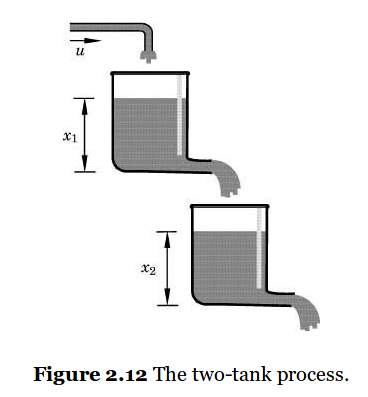
\includegraphics[width=\linewidth]{../../figures/fig2-12-two-tank-system.png}
\end{minipage}


\begin{enumerate}
\item Determine an observer with poles that are twice as fast as the fastest mode of the plant.
\item Determine a state feedback gain \(L\) such that the closed-loop system has poles in \( 0.8 \pm 0.1\).
\end{enumerate}

\begin{center}
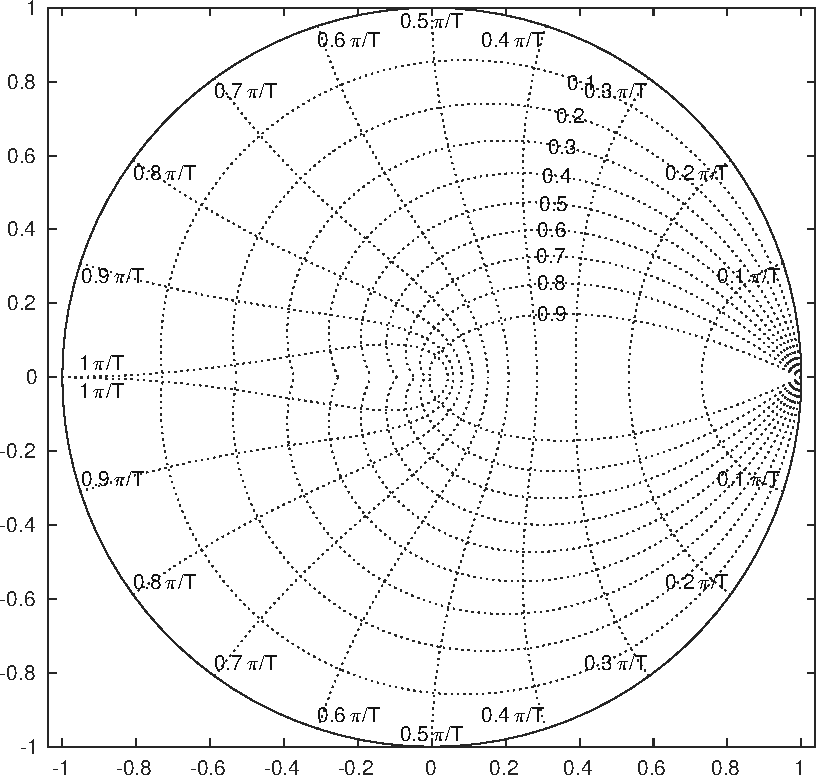
\includegraphics[width=0.45\linewidth]{../../figures/zgrid-crop}
\end{center}

\newpage 

\subsection*{Implementing the controller}
\label{sec-0-4}
Complete the pseudo-code (matlab) below for the implementation of the controller
\begin{verbatim}
% The plant model
n = 2;
h = 12; 
Phi = [0.79 0; 0.176 0.857]; 
Gamma = [0.281; 0.0296];
C = [0 1];

% The controller and observer gains

L = 

K = 

% Initialize variables
u = 0; xhat = [0; 0];
% Run the controller 
while run_controller() % The function run_controller will return 0 if the controller should stop
   y = get_output();  % Returns the sampled output signal from the plant
   uc = get_setpoint();  % Returns the desired water leve in the second tank

   % Update the observer

   xhat = 

   % Compute the control signal

   u = 

   % Send the control signal to the plant
   write_control_signal(u);
   % Wait until next sampling instant
   sleep(h); % Assuming that the computational time is negligable
end
\end{verbatim}


\section*{Solution}
\label{sec-1}

\begin{enumerate}
\item The estimation error of the observer satisfies the difference equation
\[ \tilde{x}(kh+h) = \left( \Phi - KC \right) \tilde{x}(kh). \]
We can choose the poles of the matrix \( \Phi - KC\) freely if the system is \textbf{observable}. Here we have
\[ W_o = \bbm C\\ C \Phi \ebm = \bbm 0 & 1\\ 0.176 & 0.857 \ebm, \]
so \(\det W_o = -0.176 \neq 0\), i.e. the system is \textbf{observable}.

The poles of the continuous-time plant are \(-0.0197\)  and \(-0.0129\). The fastest poles is thus \(-0.0197\). The discrete-time observer poles should be twice as fast. This is obtained by placing the observer poles in 
\[ \mexp{2(-0.0197)h} \approx 0.62. \]
Verify by studying the z-plane grid. This gives the desired characteristic polynomial 
\[ (z-0.62)^2 = z^2 - 1.24z + 0.3844 \] for the observer.

We have
\begin{equation*}
\begin{split}
\Phi - KC &= \bbm 0.790 & 0\\ 0.176 & 0.857 \ebm - \bbm k_1\\k_2 \ebm \bbm 0 & 1 \ebm\\
&= \bbm 0.790 & 0\\ 0.176 & 0.857 \ebm - \bbm 0 & k_1\\ 0 & k_2 \ebm\\
&= \bbm 0.790 & -k_1\\ 0.176 & 0.857-k_2 \ebm.
\end{split}
\end{equation*}
Which gives the characteristic polynomial
\begin{equation*}
\begin{split}
\det \left( zI - (\Phi - KC) \right) &= \det \bbm z - 0.790 & k_1\\ -0.176 & z-0.857+k_2 \ebm \\
&= (z-0.790)(z-0.857+k_2) + 0.176k_1 = z^2 + (-0.790-0.857+k_2)z -0.790(-0.857+k_2) 0.176k_1\\
&= z^2 + (k_2 -1.647)z + 0.176k_1 - 0.790 k_2 + 0.677
\end{split}
\end{equation*}

Setting the coefficients of the two characteristic polynomials equal gives the system of equations
\begin{align*}
k_2 - 1.647 &= -1.24 \quad \Rightarrow \quad k_2 = 0.407\\
0.176k_1 - 0.790 k_2 + 0.677 &= 0.3844 \quad \Rightarrow \quad k_1 \approx 0.164.
\end{align*}

\item Now design the feedback gain \(L\). The system  is \textbf{reachable} since 
\[W_c = \bbm \Gamma & \Phi\Gamma \ebm = \bbm 0.281   &  0.222 \\ 0.0296 & 0.0748  \ebm \]
\[ \det W_c = 0.0145 \neq 0\].

The desired characteristic polynomial is 
\[ (z - 0.8 -0.1i)(z-0.8+0.1i) = z^2 -1.6z + 0.65. \]

The closed-loop system characteristic polynomial is obtained by
\[ \det \left(zI - (\Phi - \Gamma L) \right). \]
with 
\[ \Gamma L = \bbm 0.281\\ 0.0296 \ebm \bbm l_1 & l_2 \ebm = \bbm 0.281 l_1 & 0.281 l_2\\ 0.0296 l_1 & 0.0296 l_2 \ebm \]
we get
\begin{equation*}
\begin{split}
\det \left(zI - (\Phi - \Gamma L) \right) &= \det \bbm z - 0.790 + 0.281l_1 & 0.281 l_2\\ -0.176 + 0.0296 l_1 & z - 0.857 + 0.0296 l_2 \ebm\\
&= (z-0.790 + 0.281 l_1)(z - 0.857 + 0.0296 l_2) - (-0.176 + 0.0296 l_1)(0.281 l_2)\\
&= z^2 + (-0.790 + 0.281 l_1 - 0.857 + 0.0296 l_2)z + (-0.790 + 0.281 l_1)(-0.857 + 0.0296 l_2) + 0.049 l_2 - 0.0296 \cdot 0.281 l_1 l_2 \\
&= z^2 + (0.281 l_1 + 0.0296 l_2 - 1.647)z + 0.677 - 0.023l_2 - 0.241 l_1 + 0.0296 \cdot 0.281 l_1 l_2 + 0.049 l_2 - 0.0296 \cdot 0.281 l_1 l_2 \\
&= z^2 + (0.281 l_1 + 0.0296 l_2 - 1.647)z + 0.677 - 0.241 l_1 + 0.026 l_2.
\end{split}
\end{equation*}
Setting the coefficients of the two characteristic polynomials equal gives the system of equations
\begin{align*}
0.281 l_1 + 0.0296 l_2 &= -1.6 + 1.647\\
-0.241 l_1 + 0.026 l_2 &= 0.65 - 0.677
\end{align*}
or 
\[ \bbm 0.281 & 0.0296\\-0.241 & 0.026 \ebm \bbm l_1\\l_2 \ebm = \bbm 0.047\\-0.027 \ebm \]
with solution
\[ \bbm l_1\\l_2 \ebm = \frac{1}{0.281\cdot 0.026 + 0.241\cdot 0.0296} \bbm 0.026 & -0.0296\\0.241 & 0.281 \ebm \bbm 0.047\\ -0.027 \ebm = \bbm 0.14\\0.26 \ebm. \]
\end{enumerate}
% Emacs 25.3.50.2 (Org mode 8.2.10)
\end{document}